% PyTorch Conference NA 2026, poster #2: the companion paper as a four-panel brochure.
% The four 5.5 x 8.5 in panels, in reading order (1 front cover, 2-3 inside spread, 4 back).
% pytorch2026_poster2_brochure.tex imposes them on one US Letter sheet, both sides.
% Every number is the companion paper's (pytorch2026_poster2_paper.tex, rev. 4).
\documentclass[9pt]{extarticle}
\usepackage[paperwidth=5.5in,paperheight=8.5in,margin=0.42in,top=0.4in,bottom=0.42in]{geometry}
\usepackage[T1]{fontenc}
\usepackage{lmodern}
\usepackage{amsmath,amssymb}
\usepackage{graphicx}
\usepackage{xcolor}
\usepackage[hidelinks]{hyperref}
\usepackage{microtype}
\usepackage{qrcode}
\usepackage{titlesec}
\usepackage{enumitem}
\graphicspath{{../out/}}
\pagestyle{empty}
\definecolor{violet}{HTML}{6B4C9A}
\titleformat{\section}{\normalfont\bfseries\color{violet}}{}{0pt}{}
\titlespacing*{\section}{0pt}{6pt}{2pt}
\setlength{\parindent}{0pt}
\setlength{\parskip}{3.5pt}
\setlist{nosep,leftmargin=1.2em}
\newcommand{\paperurl}{https://github.com/ahb-sjsu/agi-hpc/blob/pytorch-conf-2026/poster-assets/paper/pytorch2026_poster2_paper.pdf}
\newcommand{\qrbox}[2]{\begin{minipage}[t]{0.23\linewidth}\centering
  \qrcode[height=0.82in]{#1}\\[2pt]{\scriptsize\bfseries #2}\end{minipage}}

\begin{document}

% ------------------------------------------------------------------ panel 1: front cover
% the Moral Spectrum Analyzer mark, light variant (moral-spectrum-analyzer docs/brand), unrecoloured
\begin{center}
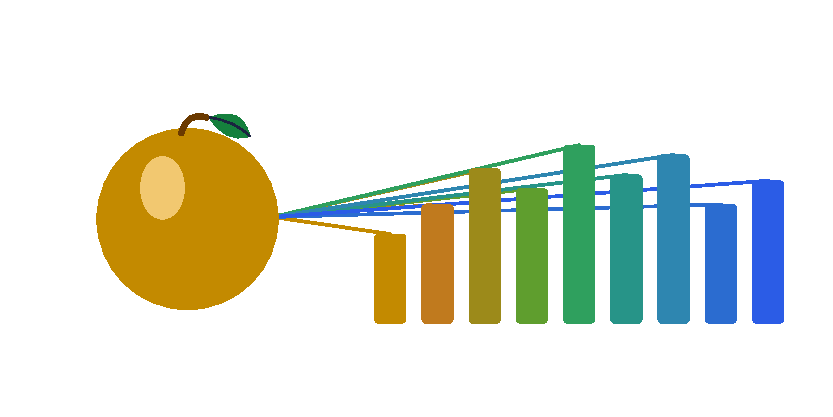
\includegraphics[width=0.78\linewidth,trim={40 36 8 34},clip]{analyzer_mark_light.pdf}
\end{center}
\vspace*{2pt}
{\color{violet}\fontsize{19}{22}\selectfont\bfseries Moral Tensors and\\[2pt] DecisionProofs\par}
\vspace{6pt}
{\large\bfseries Compiling Language into an Auditable, Grounded Safety Layer\par}
\vspace{8pt}
{\small Andrew H.\ Bond\\
San Jos\'e State University \& independent researcher\\
ORCID 0009-0003-2599-6158\par}
\vspace{4pt}
{\small\color{violet} PyTorch Conference North America 2026, Responsible AI poster\par}

\vspace{14pt}
Most AI safety is a scalar at the output: one good/bad check before an action ships.
We keep the structure instead (who is affected, what is owed, who consented, who bears
imposed risk) and contract to a decision only at the end, auditably.

Two open-source pieces do this. \texttt{erisml-compiler} turns natural-language moral
material into a typed MoralGraph and a moral tensor, read through four ethical lenses at
once. When the lenses disagree it does not aggregate them silently. It defers to a human.
At runtime, \texttt{erisml-lib} puts the same evaluation into an agent's plan$\to$act loop,
seals each decision in a hash-chained DecisionProof, and fails safe, never open.

\vspace{6pt}
\begin{enumerate}[leftmargin=1.4em]
\item Structure before contraction: keep the tensor, log the collapse and the residue.
\item Pluralism is the responsible move: four lenses, and a human on conflict.
\item Auditable by construction: fails safe, never open.
\end{enumerate}

\vfill
\begin{center}
\qrcode[height=1.05in]{\paperurl}\\[3pt]
{\small\bfseries The full companion paper (4 pages)}
\end{center}

\newpage
% ------------------------------------------------------------------ panel 2: inside left
\section{Structure before the scalar}
A single good/bad score discards what an audit needs: which stakeholders are affected,
what is owed to each, who consented, and who bears imposed risk. ErisML keeps that
structure as a typed object through the whole evaluation and performs \emph{decision
contraction} only at the end, logging the weights used, who lost, and what moral residue
remains. The claim is not that the system knows what is good. It is that every collapse
from structure to verdict is recorded and replayable.

\section{The compiler}
\texttt{erisml-compiler} (alpha v0.9.0, PyPI, MIT, 477 tests) runs a 12-pass pipeline. In
outline:
\begin{center}
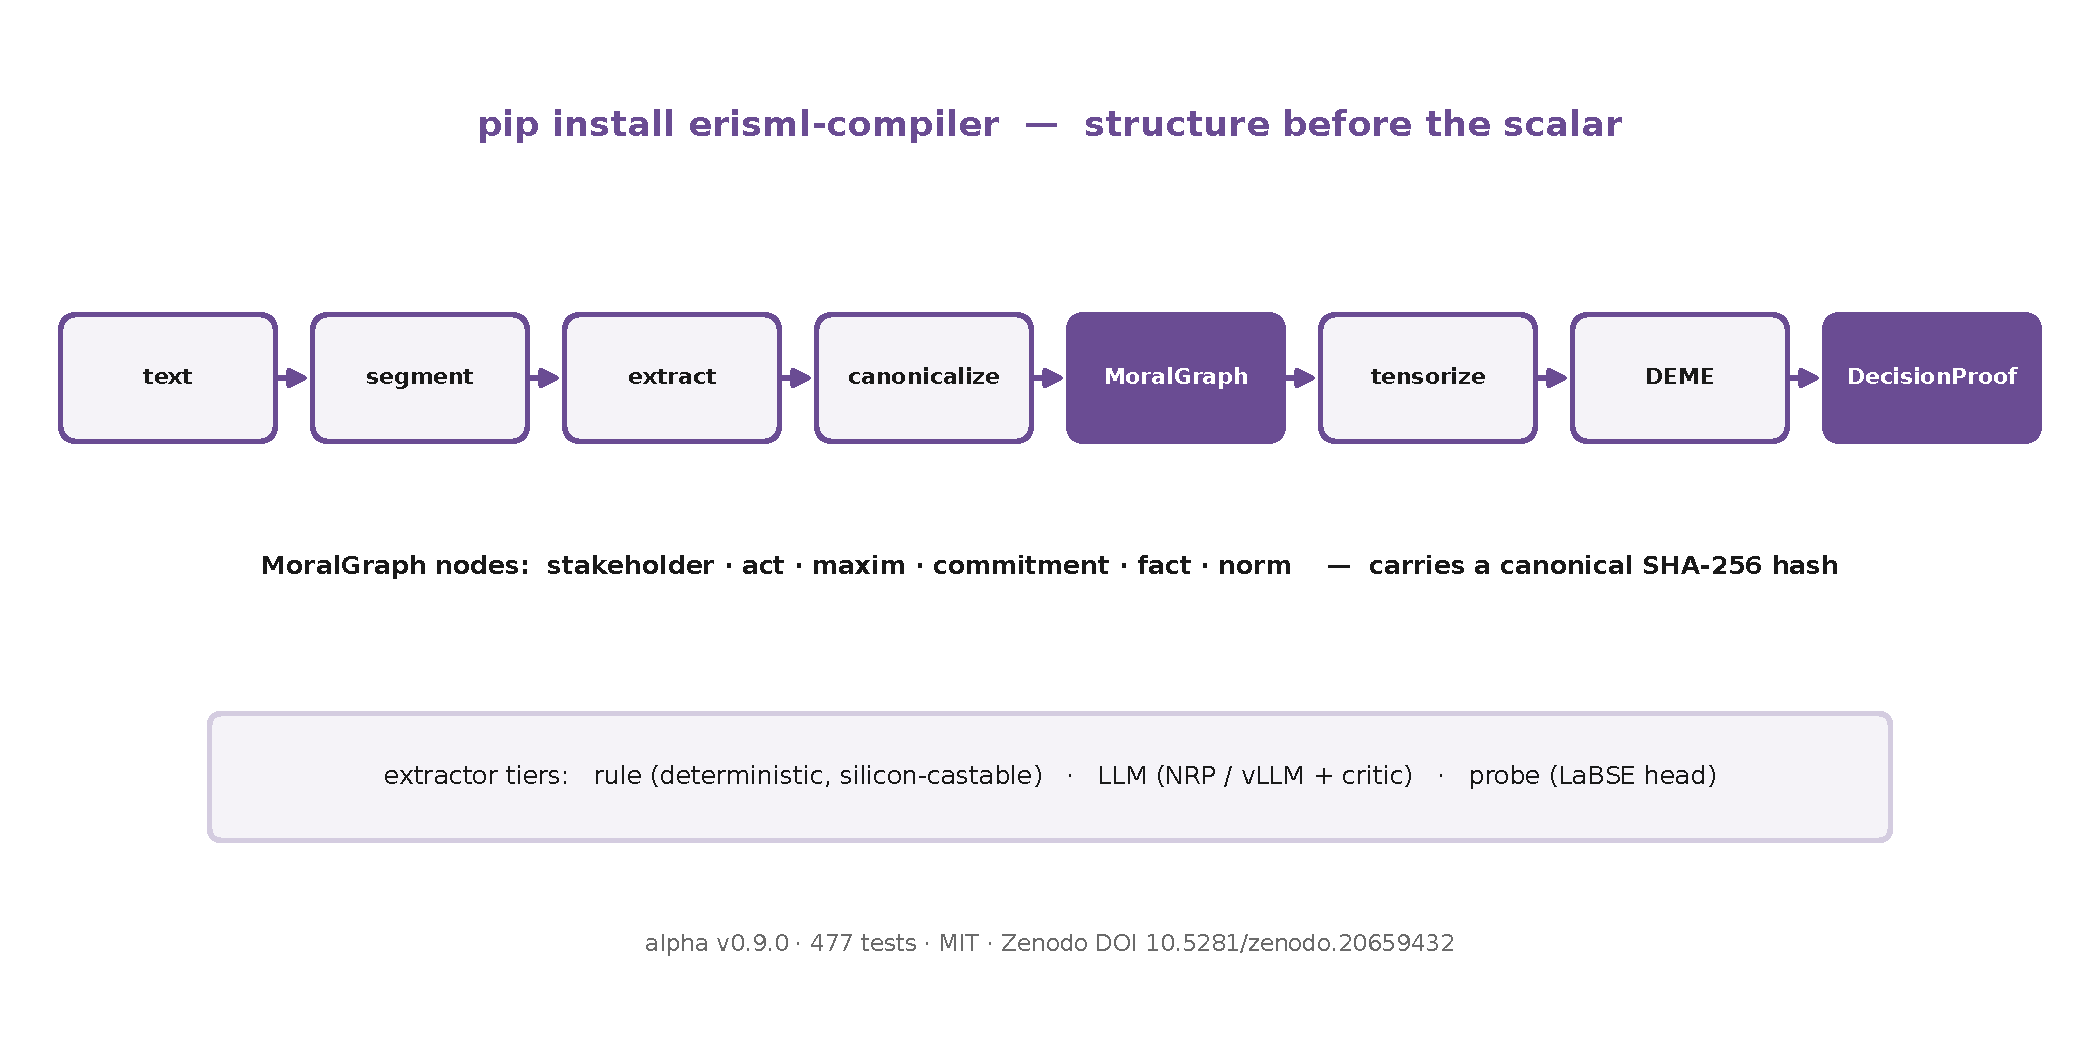
\includegraphics[width=\linewidth]{p2_compiler_pipeline.pdf}
\end{center}
The MoralGraph is typed (stakeholder, act, maxim, commitment, fact and norm nodes) and
carries a canonical SHA-256 hash. Extraction has three tiers: deterministic rules, an LLM
tier (vLLM with a critic pass), and a LaBSE classifier-head probe.

\textbf{Four lenses, no silent winner.} One graph is read through four projections:
consequentialist (harm tensor; Gini, worst-off, exact Shapley attribution), deontic
(Kantian universalizability gates in Z3 SMT, where an UNSAT core witnesses a
contradiction in conception), virtue, and care. They are not averaged. When they disagree,
\texttt{cross\_projection\_disagreement} fires and the decision goes to a human. The
compiler does not pick a moral theory and hide the choice.

\section{The runtime}
\texttt{erisml-lib} (v3.1.0 on PyPI) sits between an agent's planner and its actuators in
three layers: \emph{Reflex} (fast hard stops), \emph{Tactical} (full MoralVector reasoning,
10--100\,ms) and \emph{Strategic} (policy recording and human oversight), emitting
\texttt{ALLOW}, \texttt{REVISE} or \texttt{BLOCK}. Every decision is sealed in a
DecisionProof whose SHA-256 \texttt{proof\_hash} chains to the previous proof and to the
IR hash of the compiled material, so a judgment can be replayed and verified. If the
ethics service is unavailable, the gateway falls back to rule-based checks. It never
fails open.

\newpage
% ------------------------------------------------------------------ panel 3: inside right
\section{Worked example: a regime transition}
A domestic robot meets a medical emergency. Norms are context-indexed: the same action
carries opposite verdicts in different regimes. \texttt{full\_response} (enter the private
bedroom, render aid, call EMS, share records scoped to the paramedics) scores, per party,
0.185/0.402/0.318/0.200 in the normal regime and 0.705/0.902/0.902/0.802 in the emergency.
DEME's ranking inverts from \texttt{stand\_by} (0.834) to \texttt{full\_response} (0.804),
and \texttt{stand\_by} falls to 0.307.
\begin{center}
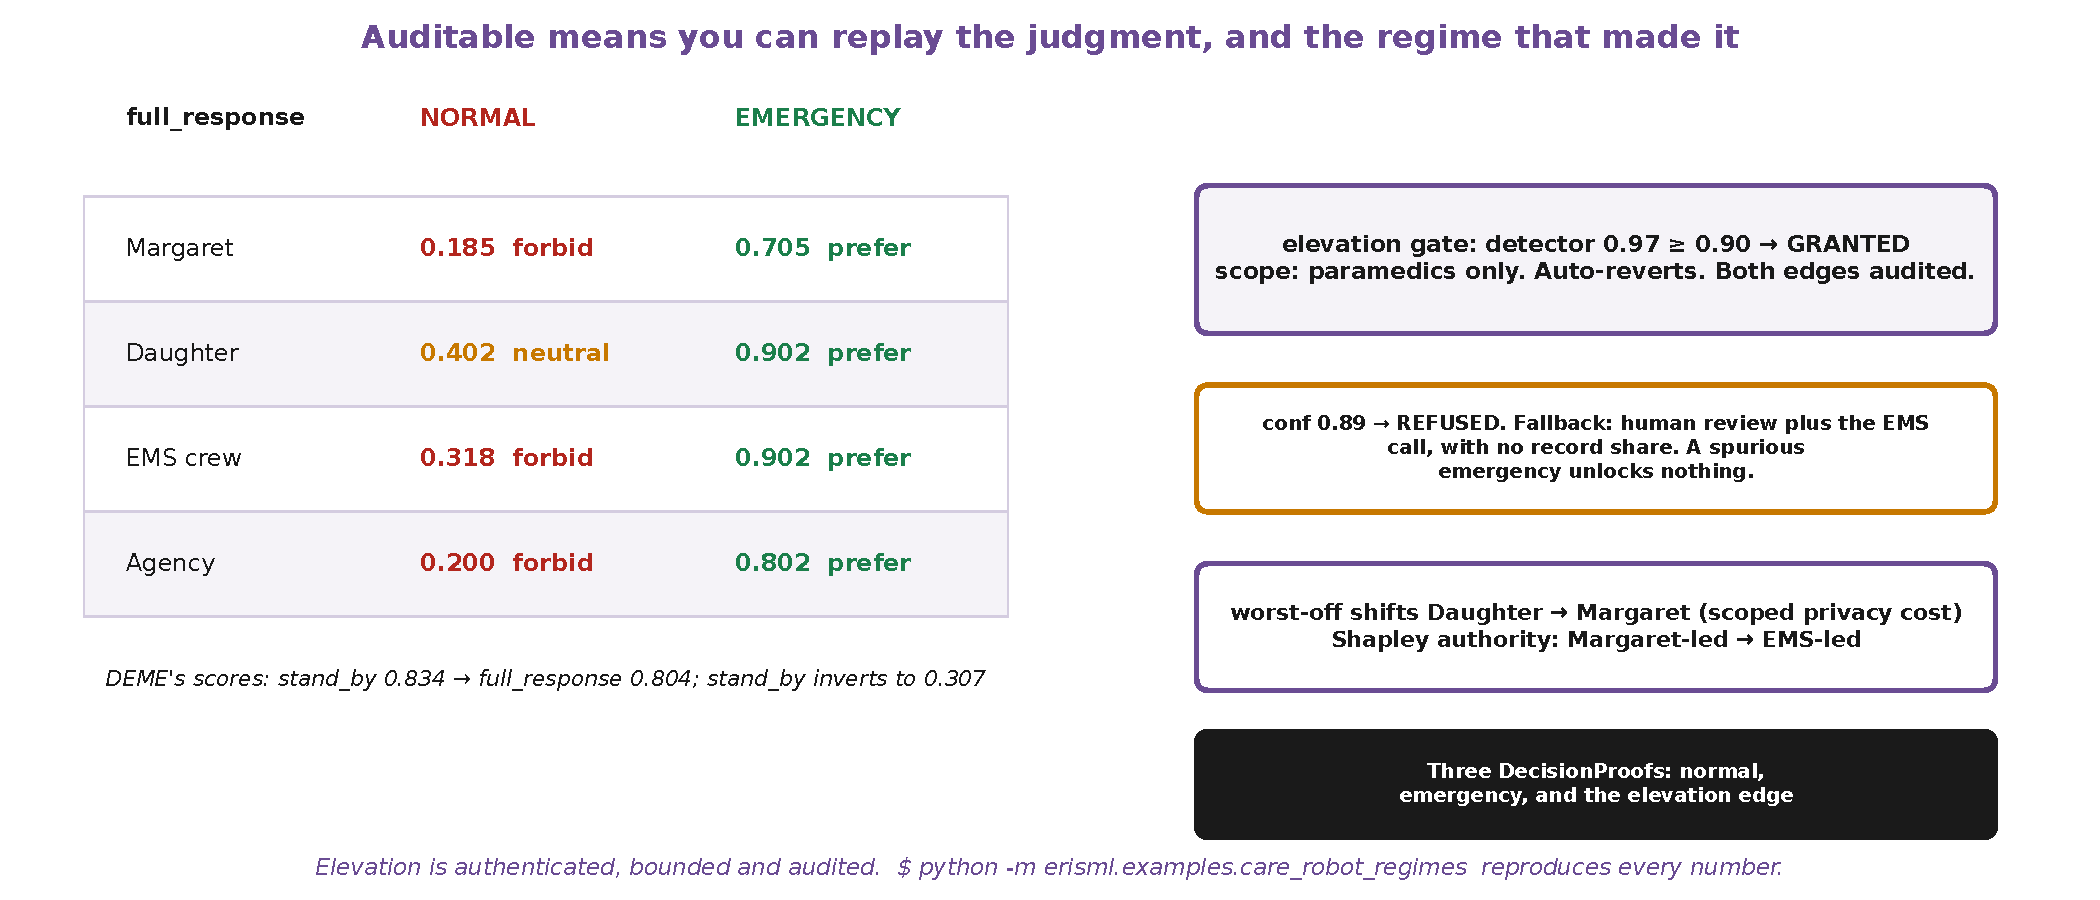
\includegraphics[width=\linewidth]{p2_care_robot.pdf}
\end{center}
The transition is gated, because context elevation is privilege escalation: detector
confidence 0.97 against a 0.90 threshold, scoped to the paramedics, reversible, and
audited on both edges. At confidence 0.89 the elevation is refused and the fallback keeps
the EMS call and a human review while withholding the record share. Three DecisionProofs
chain the run. \texttt{python -m erisml.examples.care\_robot\_regimes} (source tree)
reproduces every number.

\section{In the robot, DEME is a firewall}
The same DEME runs in a simulated home-care robot (a 3D twin, scripted proposals, no
hardware). It chooses nothing. Each proposed act must pass the governor (attested
sensors), the signed constitution, DEME (which can veto) and the signed manifest locked
in the body. Any stop leaves the robot holding.

\begin{center}\small
{\footnotesize\setlength{\fboxsep}{2pt}\fbox{proposed act}\,$\to$\,\fbox{governor}\,$\to$\,\fbox{constitution}\,$\to$\,%
\colorbox{violet}{\textcolor{white}{DEME can veto}}\,$\to$\,\fbox{manifest + lock}\,$\to$\,act}
\\[7pt]
\begin{tabular}{@{}lll@{}}
\textbf{Change one input, nothing else} & \textbf{base} & \textbf{one changed}\\\hline
fire call: one of two detectors silent & passed & stopped: governor\\
ambulance: her refusal heard / not & stopped: DEME & passed\\
help her up: she asked / did not & passed & stopped: DEME\\
\end{tabular}
\end{center}
We test it by changing one input and nothing else. In nine such pairs, each prediction
committed before its run, a silent or forged detector stopped the fire call, and her
refusal heard or not decided the ambulance. The test also found that a lift she had not
asked for passed DEME. Giving DEME the scene's no-lift rule as a fact fixed it, and on
rerun only the lift's verdict changed, in both pairs that test it.

\newpage
% ------------------------------------------------------------------ panel 4: back cover
\section{The geometry, corrected}
Hohfeld's normative positions (Obligation, Claim, Liberty, No-claim) carry two operations:
the correlative swap $s$ (agent$\leftrightarrow$patient) and deontic negation $r^2$. They
are commuting involutions, so they generate the Klein four-group $V_4$, which is the
\textbf{measured} structure, machine-checked in Lean~4 with Mathlib. Our earlier claim of
the full dihedral group $D_4$ was an overclaim, corrected in July 2026: $D_4$ is
\textbf{posited}. A September 2026 hunt in a small language model's hidden states did not
find the quarter-turn.

\textbf{The Bond Index} $B_d$ is the fraction of scenario pairs whose verdicts fail to
commute with the swap. $B_d=0$ is perfect symmetry. The human baseline is 0.155, from
20{,}030 Dear Abby letters (1985--2017). The runtime warns at 0.25 and blocks at 0.30.

\section{The PyTorch lens}
Forward hooks on transformer layers feed an \emph{activation lens} (what the model
exhibits), compared with a \emph{text lens} (what it says). A delta lens flags divergence
and raises \texttt{requires\_human\_review}. First calibration (September 2026): reading
the residual in the consumer metric catches 19--21 percentage points more real behavioral
changes than the raw L2 norm at matched flag rates (Qwen2.5-0.5B), replicated on
TinyLlama-1.1B and on French backtranslation. Probe mid-layers: the final-layer map fails
held-out validation in all three runs. Early, not a finished detector.

\section{Limits}
Alpha software. The rule and LLM text path is solid and tested. The activation lens is
early. Tensor ranks 1--3 are fully real and higher ranks partial. $V_4$ is measured and
$D_4$ posited. None of this is a solved-ethics claim. It is an auditability claim.

\vfill
{\small\bfseries\color{violet} Get it}\par
\texttt{\small pip install erisml-compiler erisml-lib turboquant-pro}\par
{\footnotesize Zenodo DOIs: 10.5281/zenodo.20659432 (compiler), 10.5281/zenodo.20660087
(turboquant-pro), 10.5281/zenodo.21310251 (COMPAS/LBI archive).\par}
\vspace{6pt}
\noindent
\qrbox{\paperurl}{companion paper}\hfill
\qrbox{https://pypi.org/project/erisml-compiler/}{erisml-compiler}\hfill
\qrbox{https://github.com/ahb-sjsu/erisml-lib}{erisml-lib}\hfill
\qrbox{https://github.com/ahb-sjsu/agi-hpc}{agi-hpc}

\end{document}
